% !TEX root = ../manuscript.tex

\chapter{Dynamical Systems on Lie Groups}

Having defined derivatives on Lie Groups we can introduce dynamical systems that evolve on Lie Groups. ODEs can be defined in multiple ways depending on how derivatives are handled. Consider a system $\X(t)$ whose state can be interpreted as a mapping $\mathbb{E}(1) \rightarrow \cM$.

If $^\X \a$ is the body derivative the system can be written with an equation involving the right derivative:
\begin{equation}
  \mathrm{d}^r \X_t = {^\X}\a(t), \quad {^\X}\a(t) \in T_\X \cM.
\end{equation}
The same system can be written in terms of the derivative ${^\id}\a(t)$ in the global tangent frame $T_\id \cM$ using the left derivative:
\begin{equation}
  \mathrm{d}^l \X_t = {^\id}\a(t), \quad {^\id}\a(t) \in T_\id \cM.
\end{equation}
We can also write the global derivative as
\begin{equation}
  \mathrm{D} \X_t = \X \circ {^\X}{\hat\a}(t) = {^\id}{\hat\a}(t) \circ \X,
\end{equation}
where the derivative is with respect to the coefficients of the matrix $\X$. Naturally, as long as
\begin{equation}
  \label{eq:velocity_at_identity}
  {^\id \a(t)} = \bAd_{\X(t)} {^\X \a}(t)
\end{equation}
all these formulations describe the same dynamical system, which can be readily seen from \eqref{eq:derivative_trans}.

\section{Dynamical systems and the exponential map}

Consider the dynamical system $\X(t) = x_0 \circ \exp(t \a)$, evaluating the right derivative with respect to $t$ gives
\begin{equation}
  \mathrm{d}^r \X_t = \lim_{\tau \rightarrow 0} \frac{\exp(t \a)^{-1} \circ \exp((t + \tau) \a)}{\tau} = \lim_{\tau \rightarrow 0} \frac{\exp(\tau \a)}{\tau} = \a.
\end{equation}
It follows that $\X_0 \circ \exp (t \a)$ is the solution to the ordinary differential equation
\begin{equation}
  \begin{cases}
    \mathrm{d}^r \X_t = \a, \\
    \X(0) = \X_0.
  \end{cases}
\end{equation}


\todo[inline]{Show connection with formulas that map velocities in a rotating frame}

\subsection{Geometric Numerical Integration}

\todo[inline]{Geometric RK scheme}



\section{A Stabilizing Lie Group Controller}

Consider the system
\begin{equation}
  \begin{aligned}
    \mathrm{d}^r \X_t & = v \\
    \mathrm{d}^r v_t  & = u
  \end{aligned}
\end{equation}
where $u$ is a control input, and the objective of tracking a twice differentiable trajectory $\X_d(t)$ with first and second right-derivatives $v_d$ and $a_d$. Consider the error
\begin{equation}
  e_\X \coloneq \X_d \ominus_r \X,
\end{equation}
with derivative
\begin{equation}
  \mathrm{d}^r (e_\X)_t \overset{\eqref{eq:d_rminus_fst},\eqref{eq:d_rminus_snd}}= \left(\mathrm{d}^r \exp_{e_\X} \right)^{-1} \mathrm{d}^r \X_d - \left(\mathrm{d}^l \exp_{e_\X} \right)^{-1} \mathrm{d}^r \X = \left(\mathrm{d}^l \exp_{e_\X} \right)^{-1} (\bAd_{\exp(e_\X)} v_d - v).
\end{equation}
Note that $\bAd_{\exp(e_\X)} = \exp \ad_{e} = \sum_{k \geq 0} \frac{\ad_e}{k!}$ can typically be found on closed form via the usual expansion tricks. Let $e_v \coloneq \bAd_{\exp(e_\X)} v_d - v$ be the velocity error in the body frame; we then have the double intergrator-like error system
\begin{equation}
  \begin{aligned}
    \frac{\mathrm{d}}{\mathrm{d}t} e_\X & = \left(\mathrm{d}^l \exp_{e_\X} \right)^{-1} e_v,                        \\
    \frac{\mathrm{d}}{\mathrm{d}t} e_v  & = \frac{\mathrm{d}}{\mathrm{d}t} \left( \bAd_{\exp(e_\X)} v_d\right) - u,
  \end{aligned}
\end{equation}
Where we can further simplify
\begin{equation}
  \frac{\mathrm{d}}{\mathrm{d}t} \left( \bAd_{\exp(e_\X)} v_d\right) \overset{\eqref{eq:bAd_dl}}= \left[ \mathrm{d}^l \exp_{e_\X} \dot e_\X,  \bAd_{\exp(e_\X)} v_d \right] + \bAd_{\exp(e_\X)} \dot v_d = \left[ e_v,  \bAd_{\exp(e_\X)} v_d \right] + \bAd_{\exp(e_\X)} \dot v_d.
\end{equation}
If we further consider an input on the form $u = \left[ e_v,  \bAd_{\exp(e_\X)} v_d \right] + \bAd_{\exp(e_\X)} \dot v_d + k_p \textcolor{red}{\left( \mathrm{d}^l \exp_{e_\X} \right)^{-T}} e_\X + k_d e_v$ that cancels out the contribution from $v_d$ and adds PD feedback terms the closed-loop dynamics become
\begin{equation}
  \begin{aligned}
    \frac{\mathrm{d}}{\mathrm{d}t} e_\X & = \left(\mathrm{d}^l \exp_{e_\X} \right)^{-1} e_v,                                   \\
    \frac{\mathrm{d}}{\mathrm{d}t} e_v  & = -k_p \textcolor{red}{\left( \mathrm{d}^l \exp_{e_\X} \right)^{-T}} e_\X - k_d e_v.
  \end{aligned}
\end{equation}
Now consider a Lyapunov candidate function on the form
\begin{equation}
  V = \frac{k_p}{2} \| e_\X \|^2 + \frac{1}{2} \| e_v \|^2 + c \left \langle e_v, e_\X \right \rangle \geq \frac{1}{2} \begin{bmatrix} \| e_\X \| \\ \| e_v \| \end{bmatrix}^T \begin{bmatrix} k_p & -c \\ -c & 1 \end{bmatrix} \begin{bmatrix} \| e_\X \| \\ \| e_v \| \end{bmatrix},
\end{equation}
where $c$ is s.t. $k_p - c^2 \geq 0$ so that the matrix is positive definite. Its derivative evaluates to
\begin{equation*}
  \begin{aligned}
    \dot V & = k_p \left \langle e_\X, \left( \mathrm{d}^l \exp_{e_\X} \right)^{-1} e_v \right \rangle - k_p \left \langle e_v,  \textcolor{red}{\left( \mathrm{d}^l \exp_{e_\X} \right)^{-T}} e_\X \right \rangle - k_d \| e_v \|^2 + c \left \langle \dot e_v, e_\X \right \rangle + c \left \langle e_v, \dot e_\X \right \rangle \\
           & = - k_d \| e_v \|^2 - c \left \langle k_p \textcolor{red}{\left( \mathrm{d}^l \exp_{e_\X} \right)^{-T}} e_\X + k_d e_v, e_\X \right \rangle + c \left \langle e_v, \left(\mathrm{d}^l \exp_{e_\X} \right)^{-1} e_v \right \rangle                                                                                       \\
           & = -k_d \| e_v \|^2 - c k_p \| e_\X \|^2 - c k_d \left \langle e_v, e_\X \right \rangle + c \left \langle e_v, \left(\mathrm{d}^l \exp_{e_\X} \right)^{-1} e_v \right \rangle - c k_p \left \langle ( \textcolor{red}{(\mathrm{d}^l \exp_{e_\X})^{-T}} - I) e_\X , e_\X \right \rangle                                   \\
           & \leq -k_d \| e_v \|^2 - c k_p \| e_\X \|^2 + c k_d \| e_v \| \| e_\X \| + c \lambda_{\textrm{max}}\left( \left( \mathrm{d}^l \exp_{e_\X} \right)^{-1} \right) \| e_v \|^2 + c k_p \lambda_{\textrm{max}} \left( \textcolor{red}{\left(\mathrm{d}^l \exp_{e_\X} \right)^{-1}} - I \right) \| e_\X \|^2.
  \end{aligned}
\end{equation*}

\begin{itemize}
  \item Eigenvalues of $(\mathrm{d}^l \exp_{e_\X})^{-1}$ can be shown to be on the form $\frac{\lambda}{e^{\lambda} - 1} = \sum_{k=0}^\infty \frac{B_n}{n!} \lambda^n$, where $\lambda$ is an eigenvalue of $\ad_e$.
  \item Zero is always an eigenvalue of $\ad_e$ since $\ad_e e = 0$ due to it being a commutator (the corresponding eigenvalue of $(\mathrm{d}^l \exp_e)^{-1}$ is 1
  \item Often, the eigenvalues of $\ad_e$ are purely imaginary. The corresponding eigenvalues of $(\mathrm{d}^l \exp_{e_\X})^{-1}$ are
        \begin{equation}
          \frac{i \lambda}{e^{i \lambda} - 1} = \frac{i \lambda e^{-i \lambda / 2}}{e^{i \lambda / 2} - e^{- i \lambda / 2}} = \frac{i \lambda e^{-i \lambda / 2}}{2 i \sin \lambda / 2} = \lambda \frac{\cos \lambda / 2 - i \sin \lambda / 2}{2 \sin \lambda / 2} = \frac{\lambda}{2} \cot \frac{\lambda}{2} - i \frac{\lambda}{2}.
        \end{equation}
        That is, the real part is equal to $\frac{\lambda}{2}\cot \frac{\lambda}{2}$.
  \item For angular groups we should throttle the angular part of $\| e_X \|$ at $\pm \pi/2$ in order to avoid the region where the eigenvalues approach zero which otherwise would lead to sluggish convergence
\end{itemize}

The maximal real part for $\lambda \in [-\pi, \pi]$ is attained at $\lambda = 0$ and is equal to 1, as shown in Figure \ref{fig:cot_fcn}. Thus, for lie groups s.t. $\ad_\a$ has purely imaginary eigenvalues in the range $[-\pi, \pi]$ for all $\a$, it holds that $\left( \mathrm{d}^l \exp_{e_\X} \right)^{-1}$ has no eigenvalue with real absolute magnitude larger than 1.

\begin{figure}
  \begin{center}
    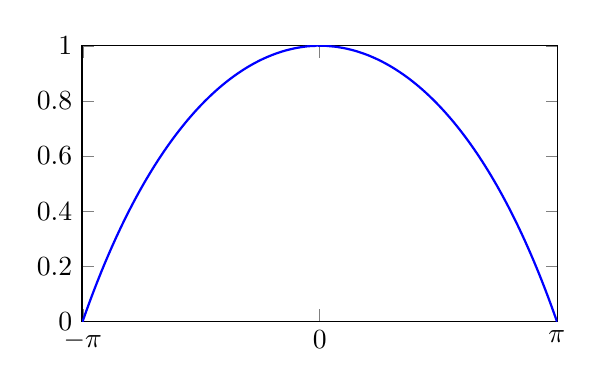
\begin{tikzpicture}
      \begin{axis}
        [
          width=3in,
          height=2in,
          xmin=-3.15,
          xmax=3.15,
          ymin=0,
          ymax=1,
          xtick={-3.14, 0, 3.1415},
          xticklabels={$-\pi$, 0, $\pi$},
        ]
        \addplot[no marks, thick, blue, samples=400]{x/2 * cot(deg(x/2))};
      \end{axis}
    \end{tikzpicture}
  \end{center}
  \caption{Function $x \mapsto \frac{x}{2} \cot \frac{x}{2}$.}
  \label{fig:cot_fcn}
\end{figure}

Let $\epsilon = \lambda_\textrm{max} \left( \textcolor{red}{\left(\mathrm{d}^l \exp_{e_\X} \right)^{-1}} - I \right)$; then we have
\begin{equation}
  \dot V \leq -\begin{bmatrix} \| e_\X \| \\ \| e_v \| \end{bmatrix}^T \begin{bmatrix} c k_p (1 - \epsilon) & -\frac{c k_d}{2} \\ -\frac{c k_d}{2} & k_d - c \end{bmatrix} \begin{bmatrix} \| e_\X \| \\ \| e_v \| \end{bmatrix}
\end{equation}
Therefore, if
\begin{equation}
  \begin{aligned}
    c k_p (1 - \epsilon) + k_d - c \geq 0 \\
    c k_p (1 - \epsilon) - \frac{c^2 k_d^2}{4}  \geq 0
  \end{aligned}
\end{equation}


\section{Sensitivity Analysis}

Consider again an ODE
\begin{equation}
  \label{eq:ode_sensitivity}
  \begin{aligned}
    \mathrm{d}^r \x_t & = f(t, \x), \\
    \x(0)             & = \x_{0}.
  \end{aligned}
\end{equation}
For a given initial condition $\x_{0}$ the solution at time $t \geq 0$ can be denoted $\phi(t; \x_{0})$ where the \emph{flow} operator $\phi : \mathbb{R} \times \M \rightarrow \M$ is s.t.
\begin{equation}
  \begin{aligned}
    \phi(0; \x_{0})                    & = \x_{0},                            \\
    \mathrm{d}^{r} \phi(t; \x_{0})_{t} & = f\left(t, \phi(t; \x_{0}) \right).
  \end{aligned}
\end{equation}

\begin{remark}
  Parameters and initial conditions are equivalent. A parameter-dependent system
  \begin{equation}
    \begin{aligned}
      \mathrm{d}^r \x_t & = f(t, \x; p_{0}), \\
      \x(t_{0})         & = \x_{0},
    \end{aligned}
  \end{equation}
  is equivalent to the parameter-free system on $\M \times \mathbb{R}^{n}$
  \begin{equation}
    \begin{aligned}
      \mathrm{d}^r (\x, p)_t & =  \left(g(t, \x, p), 0\right), \qquad g(t, \x, p) \coloneq f(t, \x; p), \\
      (\x, p)(t_{0})         & = (\x_0, p_{0}),
    \end{aligned}
  \end{equation}
  where $g(t, \x, p) = f(t, \x; p)$. Conversely, the system
  \begin{equation}
    \begin{aligned}
      \mathrm{d}^{r} \x_{t} & = f(t, \x), \\
      \x(t_{0})             & = \x_{0},
    \end{aligned}
  \end{equation}
  with a non-trivial initial condition is (locally) equivalent to the parameter-dependent system
  \begin{equation}
    \begin{aligned}
      \mathrm{d}^{r} \a_{t} & = g(t, \a; t_{0}, \x_{0}), \qquad g(t, \a; t_{0}, \x_{0}) \coloneq \left[ \mathrm{d}^{r} \exp_{\a} \right]^{-1} \; f(t_{0} + t, \x_{0} \oplus_{r} \a), \\
      \a(0)                 & = 0,
    \end{aligned}
  \end{equation}
  with trivial initial conditions, in the sense that $\Phi^{\x}(t_{0} + t; t_{0}, \x_{0}) = \x_{0} \oplus_{r} \Phi^{\a}(t; t_{0}, \x_{0})$.
\end{remark}
Due to the equivalence between parameters and initial conditions, it is sufficient to develop sensitivity for one type; we choose initial conditions as in \eqref{eq:ode_sensitivity}.

\subsection{Direct Method}

Global derivative on matrix form $\Phi = \hat \phi$.
\begin{equation}
  \dot \Phi(t; \x_{0}) = \Phi(t; \x_{0}) \left( \mathrm{d}^{r} \Phi(t; \x_{0})_{t} \right )^{\wedge} = \Phi(t; \x_{0})  \hat f\left(t, \Phi(t; \x_{0}) \right).
\end{equation}
Derivative of inverse
\begin{equation}
  \begin{aligned}
    0 = \frac{\mathrm{d}}{\mathrm{d}t} \Phi(t; \x_{0}) \circ \Phi(t; \x_{0})^{-1} = \dot \Phi(t; \x_{0}) \Phi(t; \x_{0})^{-1} + \Phi(t; \x_{0}) \frac{\mathrm{d}}{\mathrm{d}t} \Phi(t; \x_{0})^{-1} \\
    \implies \; \; \frac{\mathrm{d}}{\mathrm{d}t} \phi(t; \x_{0})^{-1} = \Phi(t; \x_{0})^{-1} \dot \Phi(t; \x_{0}) \Phi(t; \x_{0})^{-1}.
  \end{aligned}
\end{equation}
We can then evaluate how $\mathrm{d}^{r} \Phi(t; \x_{0})_{t}$ depends on $t$ by moving to global derivatives and changing the order of integration.
\begin{equation*}
  \begin{aligned}
    \frac{\mathrm{d}}{\mathrm{d}t}
     & \left( \mathrm{d}^r \Phi(t; \x_0)_{\x_0} \a \right)
    = \frac{\mathrm{d}}{\mathrm{d}t} \left( \Phi(t; \x_{0})^{-1} \left. \frac{\mathrm{d}}{\mathrm{d} \tau} \right|_{\tau = 0} \Phi(t; \x_{0} \oplus \tau \a) \right)^{\vee}                                                                                                                                                                                                                                                                                      \\
     & = \left( \left( -\Phi(t; \x_{0})^{-1} \dot \Phi(t; \x_{0}) \Phi(t; \x_{0}) \right)^{-1} \frac{\mathrm{d}}{\mathrm{d}\tau} \Phi(t; \x_{0} \oplus \tau \a) +  \Phi(t; \x_{0})^{-1} \left. \frac{\mathrm{d}}{\mathrm{d}\tau} \right|_{\tau=0} \dot \Phi(t; \x_{0} \oplus \tau \a) \right)^{\vee}                                                                                                                                                             \\
     & = \left( -\hat f\left(t; \Phi(t; \x_{0})\right) \Phi(t; \x_{0})^{-1} \left. \frac{\mathrm{d}}{\mathrm{d}\tau} \right|_{\tau = 0} \Phi(t; \x_{0} \oplus \tau \a)                                                                                                                + \Phi(t; \x_{0})^{-1} \left. \frac{\mathrm{d}}{\mathrm{d}\tau} \right|_{\tau = 0} \Phi(t; \x_{0} \oplus \tau \a) \hat f(t; \Phi(t; \x_{0} \oplus \tau \a)) \right)^{\vee} \\
     & = - \left( \hat f(t; \Phi(t; \x_{0})) \left( \mathrm{d}^{r} \Phi(t; \x_{0})_{\x_{0}} \a \right)^{\wedge}
    + \left( \mathrm{d}^{r} \Phi(t; \x_{0})_{\x_{0}} \a \right)^{\wedge} \hat f(t; \Phi(t; \x_{0}))  + \left. \frac{\mathrm{d}}{\mathrm{d}\tau} \right|_{\tau = 0} \hat f(t; \Phi(t; \x_{0} \oplus \tau \a)) \right)^{\vee}                                                                                                                                                                                                                                      \\
     & = -\left[  f(t; \Phi(t; \x_{0})), \mathrm{d}^{r} \Phi(t; \x_{0})_{\x_{0}} \a\right] + \mathrm{d}^{r} f(t, \Phi(t; \x_{0}))_{\x_{0}} \a                                                                                                                                                                                                                                                                                                                    \\
     & = -\ad_{f(t; \Phi(t; \x_{0}))} \mathrm{d}^{r} \Phi(t; \x_{0})_{\x_{0}} \a + \mathrm{d}^{r} f(t, \x)_{\x = \Phi(t; \x_{0})} \mathrm{d}^{r} \Phi(t; \x_{0}))_{\x_{0}} \a.
  \end{aligned}
\end{equation*}
\begin{important}
  The sensitivity $S(t) \coloneq \mathrm{d}^r \Phi(t; \x_{0})_{\x_{0}}$ satisfies the matrix-valued ODE
  \begin{equation}
    \label{eq:sensitivity_direct}
    \begin{aligned}
      \frac{\mathrm{d}}{\mathrm{d}t} S(t) & = \left(-\ad_{f(t, \Phi(t; \x_{0}))} + \left. \mathrm{d}^{r} f_{\x} \right|_{\x = \Phi(t; \x_{0})} \right) S(t), \\
      S(0)                                & = I.
    \end{aligned}
  \end{equation}
\end{important}

\subsection{Magnus Expansion Method}

Pose that for a system $\mathrm{d}^{r} x_{t} = f(t, \x(t))$ we have that $\x(t) = \x_{0} \circ \exp \Omega(t)$. Then
\begin{equation}
  \mathrm{d}^{r} \left(x(t)\right)_{\x_{0}} = \bAd_{\exp(-\Omega(t))}
\end{equation}
and we have that $\Omega(t)$ satisfies the equation
\begin{equation}
  f(t, \x(t)) = \mathrm{d}^{r} \x_{t} = \mathrm{d}^{r} \exp_{\Omega(t)} \Omega'(t),
\end{equation}
i.e.
\begin{equation}
  \Omega'(t) = \left[ \mathrm{d}^{r} \exp_{\Omega(t)} \right]^{-1} f \left( t, \x(t) \right)
\end{equation}

\todo[inline]{This is a problem since the vector field is not invariant: this solution form can not work.}

\begin{important}
  The sensitivity with respect to the initial condition is
  \begin{equation}
    \label{eq:sensitivity_magnus}
    \mathrm{d}^{r} \Phi(t; \x_{0})_{\x_{0}} = \bAd_{\exp(-\Omega(t))}
  \end{equation}
  where $\Omega$ satisfies the ODE
  \begin{equation}
    \begin{aligned}
      \frac{\mathrm{d}}{\mathrm{d}t} \Omega(t) & = \left[ \mathrm{d}^{r} \exp_{\Omega(t)} \right]^{-1} f \left( t, \x(t) \right), \\
      \Omega(0)                                & = 0.
    \end{aligned}
  \end{equation}
  \todo[inline]{This is kind of weird because we don't differentiate $f$}
\end{important}

\subsection{Example}

\todo[inline]{Compare the two sensitivity formulations}

\begin{example}
  If $\mathrm{d}^{r} \x_{t} = f(\x) \equiv \a$, then $\x(t) = \x_{0} \exp(t \a)$ and we get
  \begin{equation}
    \mathrm{d}^{r} (\x(t))_{\x_{0}} \overset{\eqref{eq:d_composition_rght_fst}} = \bAd_{\exp(-t \a)}.
  \end{equation}

  \paragraph{Direct Formulation}
  We furthermore know from Lemma \ref{lem:d_bad_exp} that
  \begin{equation}
    \label{eq:1}
    \frac{\mathrm{d}}{\mathrm{d}t} \bAd_{\exp(-t \a)} = -\ad_{\a} \bAd_{\exp(-t \a)},
  \end{equation}
  i.e. the sensitivity equations are
  \begin{equation}
    \label{eq:13}
    \frac{\mathrm{d}}{\mathrm{d}t} S(t) = -\ad_{\a} S(t),
  \end{equation}
  which was expected from \eqref{eq:sensitivity_direct} since $f$ is constant.

  \paragraph{Magnus Formulation}

  $\Omega$ satisfies the equation
  \begin{equation}
    \label{eq:magnus_example}
    \frac{\mathrm{d}}{\mathrm{d}t} \Omega(t) = \left[ \mathrm{d}^{r} \exp_{\Omega(t)} \right]^{-1} \a, \quad \Omega(0) = 0.
  \end{equation}
  Due to the semi-group property $\exp((t + \delta) \a) \approx \exp(t \a) \circ \exp(\delta \times \mathrm{d}^{r} \exp_{t \a} \a)$, therefore $\mathrm{d}^{r} \exp_{t \a} \a = \a$, so it follows that $\Omega(t) = t \a$ is the unique solution to \eqref{eq:magnus_example} which agrees with \eqref{eq:sensitivity_magnus}.
\end{example}

%%% Local Variables:
%%% mode: latex
%%% TeX-master: "../root"
%%% End:
